\section{Conclusion}
\label{chap:conclusion}

In the paper, we propose an online algorithm minimizing non-convex loss functions aggregated from local data distributed over a network. We show the convergence of the Frank-Wolfe gap, a standard stationary measure related to non-convex functions, in both exact and stochastic gradient settings. 
Besides, we utilize our algorithm to train a sequence to sequence deep learning model to forecast indoor temperature per zone.
Experimental results from a real-life smart building data-set makes our offerings suitable for distributed setting.

\begin{comment}
We study the effect of topology between learners on forecasting indoor temperature and quite intuitively the complete graph performs robustly better.
We notice that the algorithm can be susceptible to cumulative noise and a trivial data driven method is used to eliminate bad data sources.
\end{comment}

An interesting and related direction is to study the training of a bi-directional map between two features spaces $U$ (temperature) and $V$ (AC Energy Power). The challenge stems from modelling continuous but not necessarily differentiable data like electric power consumption that usually have fast response times with sharp edges and falls.
Another interesting investigation will be the design of robust algorithm for the setting with dynamic communication graphs.  
%In a nutshell, the work adds to the future investigation of dynamic and "data-safe" network configurations without modelling the sudden drop in and out  nature due to uncertainty in networking communications.  

% This leads to a class imbalance of roughly $1:3$ between high and low power modes across 4 zones. 
% Intuitively, in a 24 hour office setting, on can be explained by 6 hours of work + 2 hours of lunch+break and remaining 16 hours of inactivity to add up to a day.


% As per our formulation, each node in the graph locally has a memory-like component called oracle that assists a deep neural network to infer predictions. 
% For every node, the knowledge federation protocol prohibits sharing of the local memory, but instead transmits gradients and deep neural network. 
% Weights from adjacent neighbours are transferred over the network to perform local updates on the oracle and assist network. 
% Herein lies the scope of further improvement with respect to communication payload, guard against adversarial attacks and model heterogeneity. 
% The communication cost can be reduced through compression techniques like quantizing the gradient or identifying important sparse gradients to transmit.
% In the current work, we do not model adversarial attacks as a test of robustness since the data come from the similar semantics governing. the smart building.
% In a connected topology of learners, it can be important to single out bad performers or bad data generation sources to preserve the sanity of performance.
% We assume that all the nodes are running structurally identical assist networks along with oracles. 
% It is interesting to study knowledge exchange between heterogeneous models and zone out regions with high information content. 
% \Future Work{Controlling AC with Ambience-Power Mapping }
% \begin{figure}%
%     \centering
%     \subfloat[\centering Effect of AC on temperature  ]{{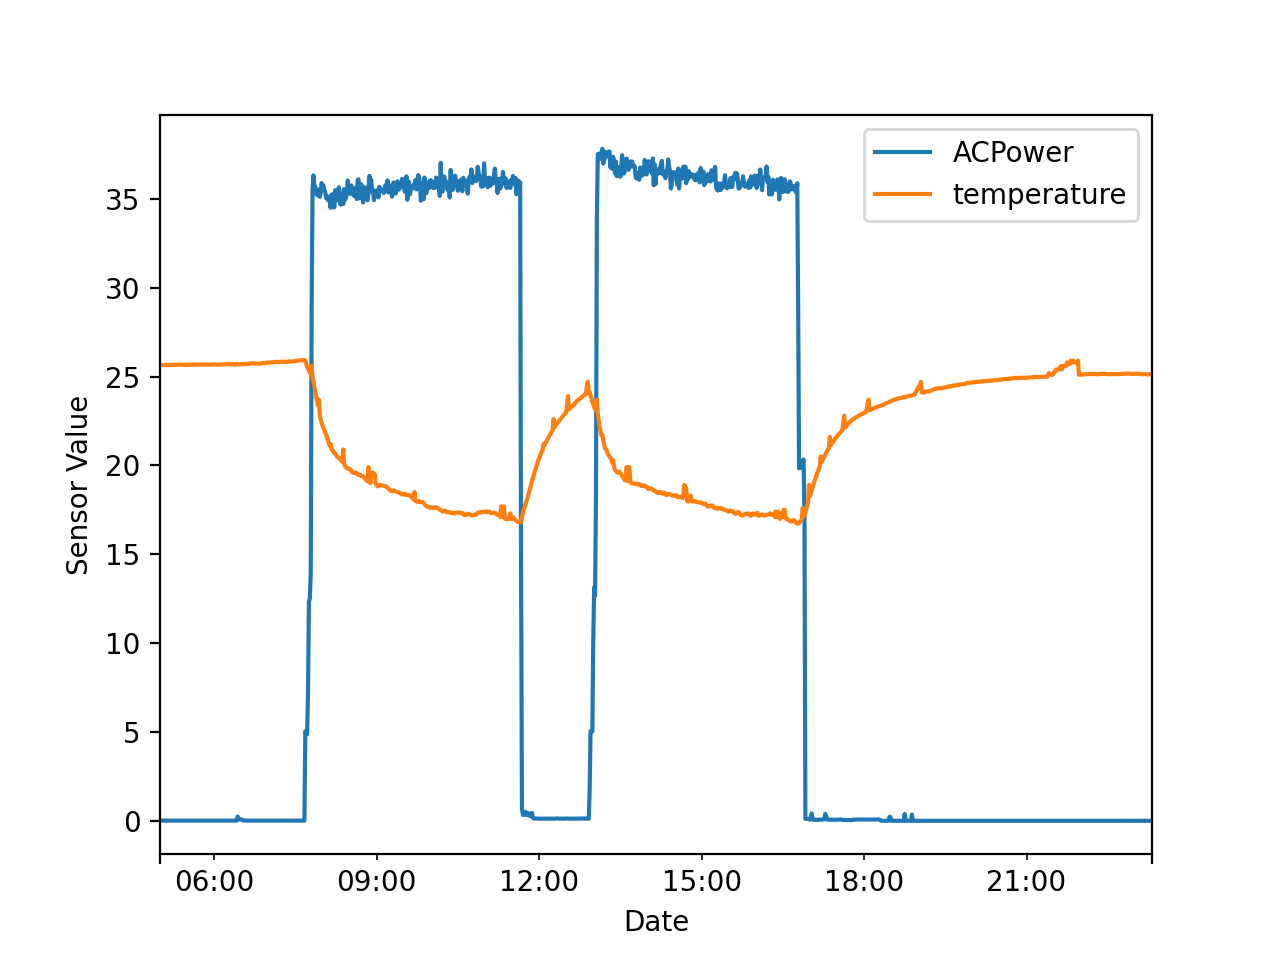
\includegraphics[width=7cm]{img/actempf7z1.png} }}%
%     \caption{ Indoor Ambience leading AC Power dissipation}%
%     \label{fig:avsp}%
% \end{figure}
% When an Air Conditioner is on, the temperature falls to a certain set point and then starts rising to equilibrium with the outdoor temperature once the device is switched off.
% Similarly, when illumination power is on, then the luminosity levels are expected to be high and low otherwise.
% Figure \ref{fig:avsp} reflects the interaction between power channels and ambient values of a zone.
% We observe that although the AC power output is continuous, the electrical device is rather controlled by a set of predefined modes. 
% We develop an online mapping $f: U \rightarrow V$ between feature spaces $(U,V)$ where $U$ is the ambient feature space and $V$ is the AC power modes.   
% This leads to a class imbalance of roughly $1:3$ between high and low power modes across 4 zones. 
% Intuitively, this can be explained by 6 hours of work + 2 hours of lunch+break and remaining 16 hours of inactivity to add up to a day.

% Table \ref{table:powerClass} shows the threshold chosen for 4 zones to bifurcate the AC power consumption into high and low modes.
% For every batch of temperature and AC Power data processed locally at each node, the oracle and deep learning model are updated L times.
% At every state of the update, the local gradients and neural network weights are send to connected neighbours. 
% Figure \ref{fig:mapPerf} gives the variation of performance metrics during L= 570 rounds of knowledge sharing. 
% The average loss in training is   [0.056] 
% The average F1 score, precision and recall are $0.881 \pm 0.15 $, $0.888 \pm 0.174$ and $0.891 \pm 0.118$ respectively.

% \begin{table}[]
% \centering
% \begin{tabular}{|l|l|l|l|l|}
% \hline
% Power Level & Floor7Z1 &Floor7Z2 & Floor7Z4 & Floor7Z5   \\ \hline
% Low Power & {[}0, 30{]} & {[}0, 25{]} & {[}0, 25{]} & {[}0, 15{]}   \\ \hline
% High Power & {[}30, 100{]} & {[}25, 100{]} &{[}25, 100{]}&{[}15, 100{]}  \\ \hline
% \end{tabular}
% \caption{Binary Classification of AC Power Levels (kW) for 4 Zones in Floor 7 }
% \label{table:powerClass}
% \end{table}

% % nb_iterations = len(train_date)*len(trainloader[0]["2019-03-08"])

% % \begin{figure}%
% %     \centering
% %     \subfloat[\centering Performance Measure  ]{{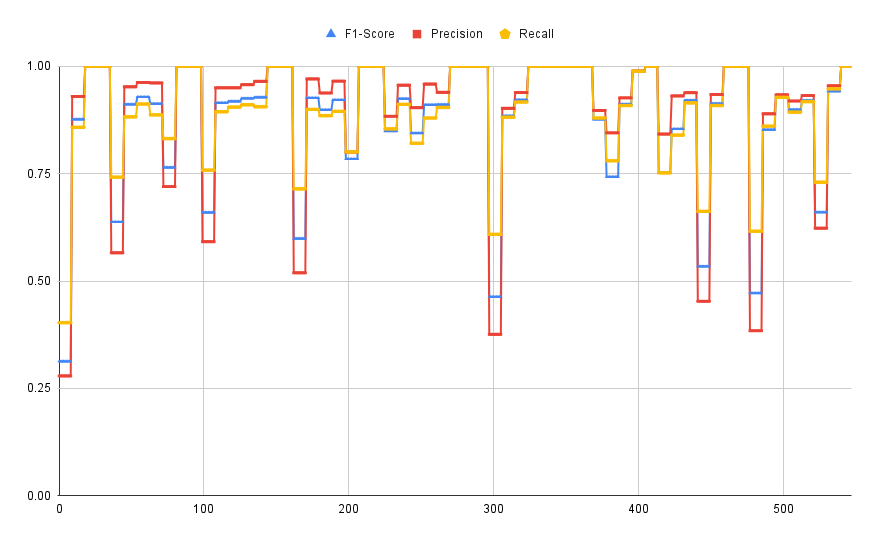
\includegraphics[width=7cm]{img/mapIterationPerformance.png}}}%
% %     \qquad
% %     \subfloat[\centering Gap Loss ]{{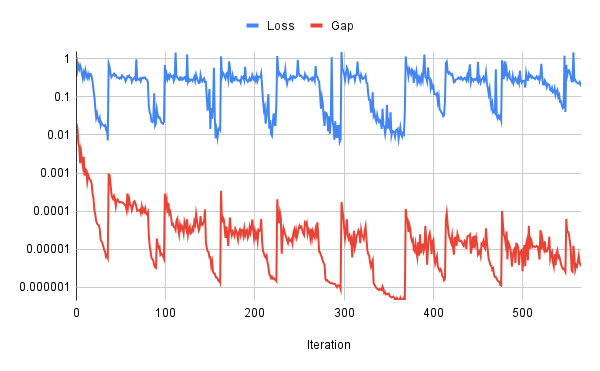
\includegraphics[width=7cm]{img/mapLossGap.png} }}%
% %     \caption{Temperature to AC Switching Mode Prediction}%
% %     \label{fig:mapPerf}%
% % \end{figure}




% % \begin{figure}%
% %     \centering
% %     \subfloat[\centering Effect of AC on temperature  ]{{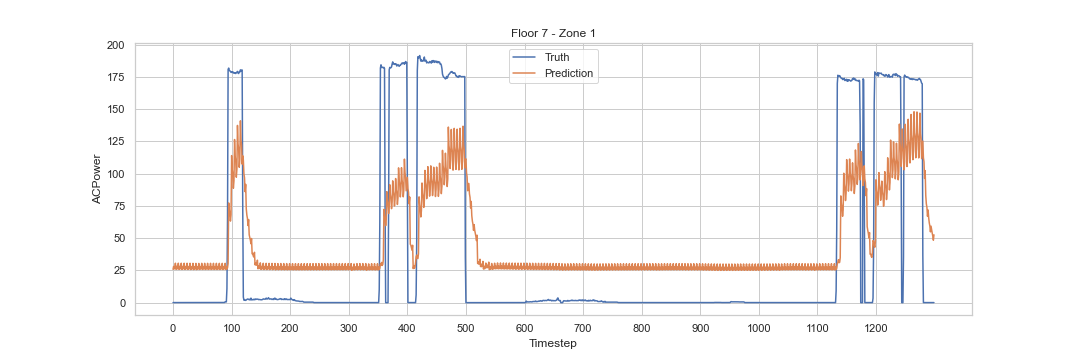
\includegraphics[width=7cm]{img/temp-ac-mapping/floor7-cycle/prediction-F7-zone1.png}}}%
% %     \qquad
% %     \subfloat[\centering Luminosity vs Light Power ]{{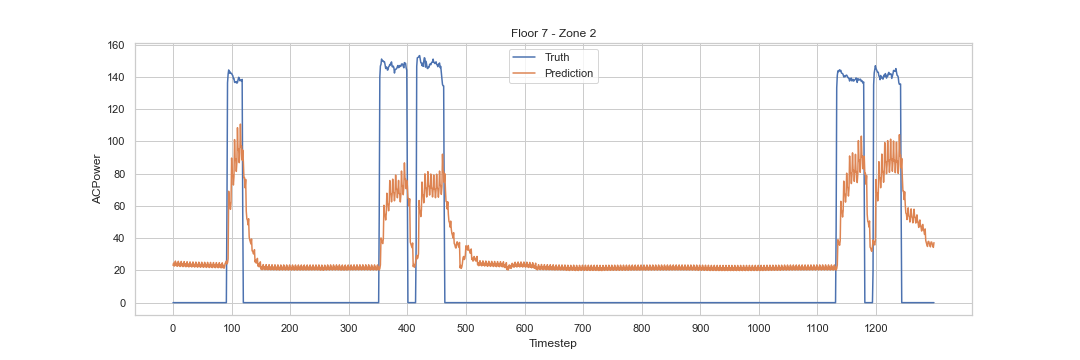
\includegraphics[width=7cm]{img/temp-ac-mapping/floor7-cycle/prediction-F7-zone2.png} }}%
% %     \qquad
% %     \subfloat[\centering Luminosity vs Light Power ]{{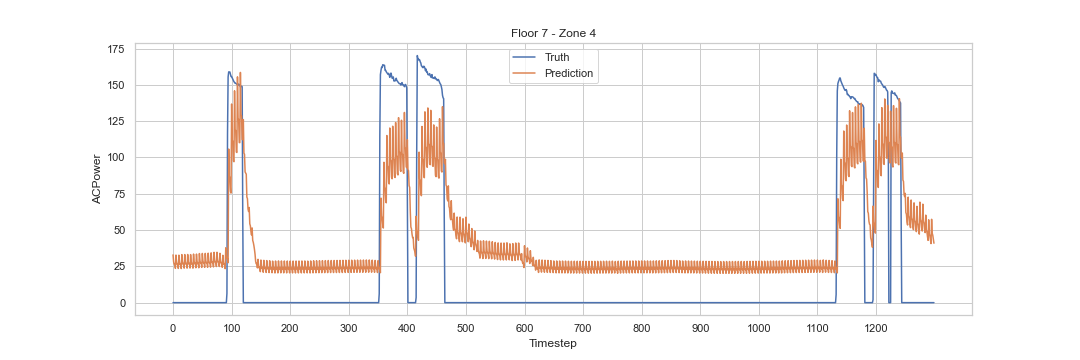
\includegraphics[width=7cm]{img/temp-ac-mapping/floor7-cycle/prediction-F7-zone4.png} }}%
% %     \qquad
% %     \subfloat[\centering Luminosity vs Light Power ]{{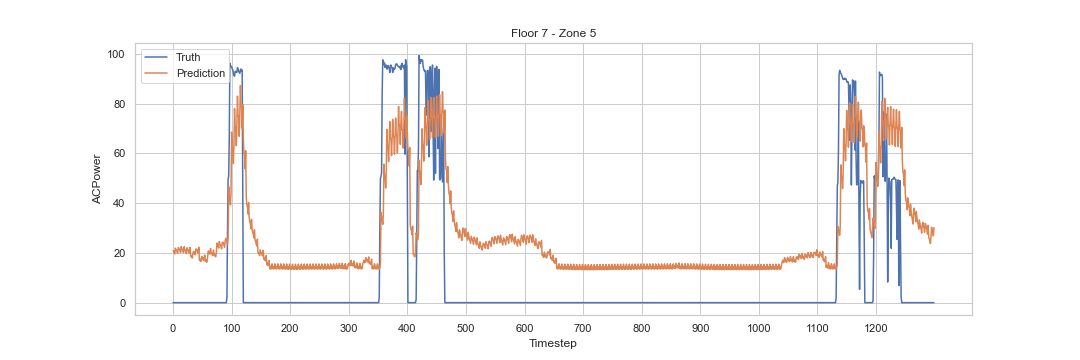
\includegraphics[width=7cm]{img/temp-ac-mapping/floor7-cycle/prediction-F7-zone5.png} }}%
% %     \caption{Temperature to AC Power on cycle graph}%
% %     \label{fig:avsp}%
% % \end{figure}

